\documentclass[12pt,letterpaper]{article}
\usepackage{graphicx,textcomp}
\usepackage{natbib}
\usepackage{setspace}
\usepackage{fullpage}
\usepackage{color}
\usepackage[reqno]{amsmath}
\usepackage{amsthm}
\usepackage{fancyvrb}
\usepackage{amssymb,enumerate}
\usepackage[all]{xy}
\usepackage{endnotes}
\usepackage{lscape}
\newtheorem{com}{Comment}
\usepackage{float}
\usepackage{hyperref}
\newtheorem{lem} {Lemma}
\newtheorem{prop}{Proposition}
\newtheorem{thm}{Theorem}
\newtheorem{defn}{Definition}
\newtheorem{cor}{Corollary}
\newtheorem{obs}{Observation}
\usepackage[compact]{titlesec}
\usepackage{dcolumn}
\usepackage{tikz}
\usetikzlibrary{arrows}
\usepackage{multirow}
\usepackage{xcolor}
\newcolumntype{.}{D{.}{.}{-1}}
\newcolumntype{d}[1]{D{.}{.}{#1}}
\definecolor{light-gray}{gray}{0.65}
\usepackage{url}
\usepackage{listings}
\usepackage{color}

\definecolor{codegreen}{rgb}{0,0.6,0}
\definecolor{codegray}{rgb}{0.5,0.5,0.5}
\definecolor{codepurple}{rgb}{0.58,0,0.82}
\definecolor{backcolour}{rgb}{0.95,0.95,0.92}

\lstdefinestyle{mystyle}{
	backgroundcolor=\color{backcolour},   
	commentstyle=\color{codegreen},
	keywordstyle=\color{magenta},
	numberstyle=\tiny\color{codegray},
	stringstyle=\color{codepurple},
	basicstyle=\footnotesize,
	breakatwhitespace=false,         
	breaklines=true,                 
	captionpos=b,                    
	keepspaces=true,                 
	numbers=left,                    
	numbersep=5pt,                  
	showspaces=false,                
	showstringspaces=false,
	showtabs=false,                  
	tabsize=2
}
\lstset{style=mystyle}
\newcommand{\Sref}[1]{Section~\ref{#1}}
\newtheorem{hyp}{Hypothesis}

\title{Problem Set 3}
\date{Due: November 11, 2024}
\author{Applied Stats/Quant Methods 1}


\begin{document}
	\maketitle
	\section*{Instructions}
	\begin{itemize}
		\item Please show your work! You may lose points by simply writing in the answer. If the problem requires you to execute commands in \texttt{R}, please include the code you used to get your answers. Please also include the \texttt{.R} file that contains your code. If you are not sure if work needs to be shown for a particular problem, please ask.
	\item Your homework should be submitted electronically on GitHub.
	\item This problem set is due before 23:59 on Sunday November 11, 2024. No late assignments will be accepted.

	\end{itemize}

		\vspace{.25cm}
	
\noindent In this problem set, you will run several regressions and create an add variable plot (see the lecture slides) in \texttt{R} using the \texttt{incumbents\_subset.csv} dataset. Include all of your code.

	\vspace{.5cm}
\section*{Question 1}
\vspace{.25cm}
\noindent We are interested in knowing how the difference in campaign spending between incumbent and challenger affects the incumbent's vote share. 
	\begin{enumerate}
		\item Run a regression where the outcome variable is \texttt{voteshare} and the explanatory variable is \texttt{difflog}.

\lstinputlisting[language=R, firstline=32, lastline=44]{PS3_JW.R} 
% Table created by stargazer v.5.2.3 by Marek Hlavac, Social Policy Institute.
% E-mail: marek.hlavac at gmail.com
% Date and time: Mon, Nov 04, 2024 - 14:15:02
\begin{table}[!htbp] \centering 
  \caption{Campaign Spending and Voteshare} 
  \label{tab:campaign_spending} 
\begin{tabular}{@{\extracolsep{5pt}}lc} 
\\[-1.8ex]\hline 
\hline \\[-1.8ex] 
 & \multicolumn{1}{c}{\textit{Dependent variable:}} \\ 
\cline{2-2} 
\\[-1.8ex] & voteshare \\ 
\hline \\[-1.8ex] 
 difflog & 0.042$^{***}$ \\ 
  & (0.001) \\ 
  & \\ 
 Constant & 0.579$^{***}$ \\ 
  & (0.002) \\ 
  & \\ 
\hline \\[-1.8ex] 
Observations & 3,193 \\ 
R$^{2}$ & 0.367 \\ 
Adjusted R$^{2}$ & 0.367 \\ 
Residual Std. Error & 0.079 (df = 3191) \\ 
F Statistic & 1,852.791$^{***}$ (df = 1; 3191) \\ 
\hline 
\hline \\[-1.8ex] 
\textit{Note:}  & \multicolumn{1}{r}{$^{*}$p$<$0.1; $^{**}$p$<$0.05; $^{***}$p$<$0.01} \\ 
\end{tabular} 
\end{table}  
The outcome of regressing difflog on voteshare cannot be interpreted easily, as difflog, meaning difference in campaign spending of incumbent and challenger party, is a logged varible. However, a positive relationship can be assumed, as the coefficient 0.042 is positive and significant at a p-value of 0.001. Consequently, one can assume, that a larger difference between campaign spending,on average has a positive effect on the voteshare of the incumbent party. 
\vspace{5cm}
		\item Make a scatterplot of the two variables and add the regression line. 	
\lstinputlisting[language=R, firstline=48, lastline=57]{PS3_JW.R} 
    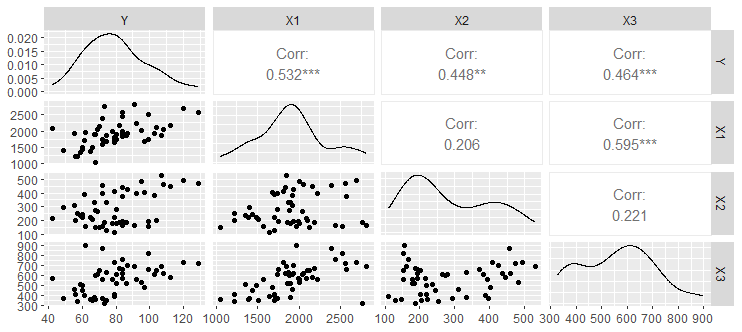
\includegraphics[width=\textwidth]{Rplot07.png}
The scatterplot shows on the Y-axis the voteshare of the incumbent, and on the X-axis the difference in campaign spending between the incumbent and the challenger. Again, a positive correlation is evident, showing that a growing difference in campaign spending increases the voteshare for the incumbent. 
		\item Save the residuals of the model in a separate object.	
\lstinputlisting[language=R, firstline=60, lastline=62]{PS3_JW.R} 

		\item Write the prediction equation
\begin{equation}
\text{voteshare} = \beta_0 + \beta_1 \times \text{difflog} + \epsilon
\end{equation}

\begin{equation}
\text{voteshare} = 0.579031 + 0.041666 \times \text{difflog} + \epsilon
\end{equation}

	\end{enumerate}
	
\newpage

\section*{Question 2}
\noindent We are interested in knowing how the difference between incumbent and challenger's spending and the vote share of the presidential candidate of the incumbent's party are related.	\vspace{.25cm}
	\begin{enumerate}
		\item Run a regression where the outcome variable is \texttt{presvote} and the explanatory variable is \texttt{difflog}.
\lstinputlisting[language=R, firstline=70, lastline=74]{PS3_JW.R} 
% Table created by stargazer v.5.2.3 by Marek Hlavac, Social Policy Institute.
% E-mail: marek.hlavac at gmail.com
% Date and time: Mon, Nov 04, 2024 - 14:28:56
\begin{table}[!htbp] \centering 
  \caption{Campaign Spending and Presvote} 
  \label{tab:campaign_presvote} 
\begin{tabular}{@{\extracolsep{5pt}}lc} 
\\[-1.8ex]\hline 
\hline \\[-1.8ex] 
 & \multicolumn{1}{c}{\textit{Dependent variable:}} \\ 
\cline{2-2} 
\\[-1.8ex] & presvote \\ 
\hline \\[-1.8ex] 
 difflog & 0.024$^{***}$ \\ 
  & (0.001) \\ 
  & \\ 
 Constant & 0.508$^{***}$ \\ 
  & (0.003) \\ 
  & \\ 
\hline \\[-1.8ex] 
Observations & 3,193 \\ 
R$^{2}$ & 0.088 \\ 
Adjusted R$^{2}$ & 0.088 \\ 
Residual Std. Error & 0.110 (df = 3191) \\ 
F Statistic & 307.715$^{***}$ (df = 1; 3191) \\ 
\hline 
\hline \\[-1.8ex] 
\textit{Note:}  & \multicolumn{1}{r}{$^{*}$p$<$0.1; $^{**}$p$<$0.05; $^{***}$p$<$0.01} \\ 
\end{tabular} 
\end{table}  
In table 2, the difference in campaign spending (difflog) is regressed on presidential voteshare (presvote). The coefficient is again not straightforward to interpret, as it remains a logged varibale, however, the positive coefficient of 0.024, significant at a p-value of 0.001 assumes a positive relationship. 
	\vspace{5cm}
		\item Make a scatterplot of the two variables and add the regression line. 
\lstinputlisting[language=R, firstline=79, lastline=88]{PS3_JW.R} 
    \includegraphics[width=\textwidth]{Rplot08.png}
This scatterplot shows the Voteshare of the presidential candidate on the Y-axis, and the differences in campaign spending between the challanger and the incumbent on the X-axis. One can assume from this data, that a larger gap in campaign spending, increases the voteshare of the presidential candidate. 
	\vspace{5cm}
		\item Save the residuals of the model in a separate object.	
\lstinputlisting[language=R, firstline=90, lastline=93]{PS3_JW.R} 
\vspace{5cm}
		\item Write the prediction equation.
\begin{equation}
\text{presvote} = 0.507583 + 0.023837 \times \text{difflog} + \epsilon
\end{equation}
	\end{enumerate}
	
	\newpage	
\section*{Question 3}

\noindent We are interested in knowing how the vote share of the presidential candidate of the incumbent's party is associated with the incumbent's electoral success.
	\vspace{.25cm}
	\begin{enumerate}
		\item Run a regression where the outcome variable is \texttt{voteshare} and the explanatory variable is \texttt{presvote}.
\lstinputlisting[language=R, firstline=101, lastline=104]{PS3_JW.R} 
% Table created by stargazer v.5.2.3 by Marek Hlavac, Social Policy Institute.
% E-mail: marek.hlavac at gmail.com
% Date and time: Mon, Nov 04, 2024 - 14:33:49
\begin{table}[!htbp] \centering 
  \caption{Presvote and Voteshare of the Incumbent} 
  \label{tab:presvote_voteshare} 
\begin{tabular}{@{\extracolsep{5pt}}lc} 
\\[-1.8ex]\hline 
\hline \\[-1.8ex] 
 & \multicolumn{1}{c}{\textit{Dependent variable:}} \\ 
\cline{2-2} 
\\[-1.8ex] & voteshare \\ 
\hline \\[-1.8ex] 
 presvote & 0.388$^{***}$ \\ 
  & (0.013) \\ 
  & \\ 
 Constant & 0.441$^{***}$ \\ 
  & (0.008) \\ 
  & \\ 
\hline \\[-1.8ex] 
Observations & 3,193 \\ 
R$^{2}$ & 0.206 \\ 
Adjusted R$^{2}$ & 0.206 \\ 
Residual Std. Error & 0.088 (df = 3191) \\ 
F Statistic & 826.950$^{***}$ (df = 1; 3191) \\ 
\hline 
\hline \\[-1.8ex] 
\textit{Note:}  & \multicolumn{1}{r}{$^{*}$p$<$0.1; $^{**}$p$<$0.05; $^{***}$p$<$0.01} \\ 
\end{tabular} 
\end{table}  
In table 3, the voteshare of the presidential candidate of the incumbent (presvote) is regressed on the voteshare of the incumbent party (voteshare). Here, the coefficient is 0.388 and significant at a p-value of 0.013. Hence, one can conclude that a one-unit increase of the presvote causes a 0.388 percent increase in voteshare, holding all else constant. Thus, the increase of the voteshare of the incumbents presidential candidate has a significant and positive effect on the incumbents electoral success overall. 
			\vspace{8cm}
		\item Make a scatterplot of the two variables and add the regression line. 
\lstinputlisting[language=R, firstline=108, lastline=117]{PS3_JW.R} 
    \includegraphics[width=\textwidth]{Rplot09.png}
This scatterplot shows the incumbents voteshare on the Y-axis, and the voteshare of the incumbents presidential candidate on the X-axis. Just as it was shown by the regression above, a positive relationship between the two varibales can be assumed.  Although strong outliners exist, made visible by the scatterplot, an upard trend of the regression line is visible. 
		\item Write the prediction equation.
\begin{equation}
\text{voteshare} = 0.441330 + 0.388018 \times \text{presvote} + \epsilon
\end{equation}
	\end{enumerate}
	

\newpage	
\section*{Question 4}
\noindent The residuals from part (a) tell us how much of the variation in \texttt{voteshare} is $not$ explained by the difference in spending between incumbent and challenger. The residuals in part (b) tell us how much of the variation in \texttt{presvote} is $not$ explained by the difference in spending between incumbent and challenger in the district.
	\begin{enumerate}
		\item Run a regression where the outcome variable is the residuals from Question 1 and the explanatory variable is the residuals from Question 2.
\lstinputlisting[language=R, firstline=124, lastline=132]{PS3_JW.R} 
% Table created by stargazer v.5.2.3 by Marek Hlavac, Social Policy Institute.
% E-mail: marek.hlavac at gmail.com
% Date and time: Tue, Nov 05, 2024 - 18:25:50
\begin{table}[!htbp] \centering 
  \caption{Regression of Residuals of Table 1 and Table 2} 
  \label{tab:residuals_regression} 
\begin{tabular}{@{\extracolsep{5pt}}lc} 
\\[-1.8ex]\hline 
\hline \\[-1.8ex] 
 & \multicolumn{1}{c}{\textit{Dependent variable:}} \\ 
\cline{2-2} 
\\[-1.8ex] & residuals\_voteshare \\ 
\hline \\[-1.8ex] 
 residuals\_presvote & 0.257$^{***}$ \\ 
  & (0.012) \\ 
  & \\ 
 Constant & $-$0.000 \\ 
  & (0.001) \\ 
  & \\ 
\hline \\[-1.8ex] 
Observations & 3,193 \\ 
R$^{2}$ & 0.130 \\ 
Adjusted R$^{2}$ & 0.130 \\ 
Residual Std. Error & 0.073 (df = 3191) \\ 
F Statistic & 476.975$^{***}$ (df = 1; 3191) \\ 
\hline 
\hline \\[-1.8ex] 
\textit{Note:}  & \multicolumn{1}{r}{$^{*}$p$<$0.1; $^{**}$p$<$0.05; $^{***}$p$<$0.01} \\ 
\end{tabular} 
\end{table}  
Table 4 shows the residuals of Table 1 (Difference in campaign spending and incumbent voteshare) regressed on the residuals of Table 2 (Differences in campaign spending and voteshare of presidential candidate). The positive coefficient of 0.257 is significant at a p-value of 0.0012, indicating that the unexplained variation in Table 1 is positively correlated with the unexplained correlatinon in Table 2. Meaning the variation within Table 1 and 2, which was not explained by the variation of their respective dependent varibales, is positively correlated with each other. 
	\vspace{6cm}
		\item Make a scatterplot of the two residuals and add the regression line. 	
\lstinputlisting[language=R, firstline=135, lastline=147]{PS3_JW.R} 
    \includegraphics[width=\textwidth]{Rplot10.png}
This scatterplot shows the residuals of Table 1 on the Y-axis and the residuals of Table 2 on the X-axis. However, contrary to the output of the regression conducted above, a slight negative correlation is visible in this scatterplot, as the regression line seems to have a negative slope. This scatterplot is possibly caused by a computational mistake of mine, which I could not deteced, although I ran the tests multiple times and double checked using the correct data.  
\vspace{6cm}
		\item Write the prediction equation.
\begin{equation}
\text{residuals\_voteshare} = -5.934 \times 10^{-18} + 0.2569 \times \text{residuals\_presvote} + \epsilon
\end{equation}
	\end{enumerate}
	
	\newpage	

\section*{Question 5}
\noindent What if the incumbent's vote share is affected by both the president's popularity and the difference in spending between incumbent and challenger? 
	\begin{enumerate}
		\item Run a regression where the outcome variable is the incumbent's \texttt{voteshare} and the explanatory variables are \texttt{difflog} and \texttt{presvote}.	
\lstinputlisting[language=R, firstline=154, lastline=159]{PS3_JW.R} 
% Table created by stargazer v.5.2.3 by Marek Hlavac, Social Policy Institute.
% E-mail: marek.hlavac at gmail.com
% Date and time: Mon, Nov 04, 2024 - 14:41:26
\begin{table}[!htbp] \centering 
  \caption{Multivariate Model: Difflog and Presvote on Voteshare} 
  \label{tab:multivariate_model} 
\begin{tabular}{@{\extracolsep{5pt}}lc} 
\\[-1.8ex]\hline 
\hline \\[-1.8ex] 
 & \multicolumn{1}{c}{\textit{Dependent variable:}} \\ 
\cline{2-2} 
\\[-1.8ex] & voteshare \\ 
\hline \\[-1.8ex] 
 difflog & 0.036$^{***}$ \\ 
  & (0.001) \\ 
  & \\ 
 presvote & 0.257$^{***}$ \\ 
  & (0.012) \\ 
  & \\ 
 Constant & 0.449$^{***}$ \\ 
  & (0.006) \\ 
  & \\ 
\hline \\[-1.8ex] 
Observations & 3,193 \\ 
R$^{2}$ & 0.450 \\ 
Adjusted R$^{2}$ & 0.449 \\ 
Residual Std. Error & 0.073 (df = 3190) \\ 
F Statistic & 1,302.947$^{***}$ (df = 2; 3190) \\ 
\hline 
\hline \\[-1.8ex] 
\textit{Note:}  & \multicolumn{1}{r}{$^{*}$p$<$0.1; $^{**}$p$<$0.05; $^{***}$p$<$0.01} \\ 
\end{tabular} 
\end{table}  
Table 5 shows a multivariate model, where the two independent variables difflog (Differences in campaign spending) and presvote (voteshare of the incumbent presidential candidate) are regressed on voteshare (voteshare of the incumbent). As in previous models, the correlation coefficients of difflog and presvote are positive and significant with 0.036 at 0.001 a alpha level, and 0.257 at a 0.012 alpha level respectively. However, again the coefficient of difflog cannot be directly interpreted as this varibale is logged, and the coefficient of presvote can be interpreted following the standard interpretation of regression outputs. 
\vspace{5cm}
		\item Write the prediction equation.	
\begin{equation}
\text{voteshare} = 0.4486442 + 0.0355431 \times \text{difflog} + 0.2568770 \times \text{presvote} + \epsilon
\end{equation}
		\item What is it in this output that is identical to the output in Question 4? Why do you think this is the case?
	\end{enumerate}
In the outputs of Question 4 and Question 5, the coefficient for residual presvote and presvote is identical (approximately 0.257). This similarity occurs because, in both cases, we are capturing the effect of presvote on voteshare while accounting for difflog. In Question 4, this effect is isolated by using residuals (the unexplained variation in voteshare and presvote after controlling for difflog), while in Question 5, it is calculated through a direct multiple regression. According to the Frisch-Waugh-Lovell theorem, these approaches yield the same coefficient for presvote since they both effectively control for difflog, allowing us to observe the unique contribution of presvote to voteshare.



\end{document}
